\documentclass[a4paper,10pt]{article}
\usepackage[utf8]{inputenc}
\usepackage{subfiles}
\usepackage{lipsum}
\usepackage{caption}
\usepackage{graphicx}
\usepackage{url}
\usepackage{tikz}
\usepackage{verbatim}
\usepackage{listings}
\usepackage{color}
\usepackage{forest}
\usepackage{adjustbox}
\usepackage{smartdiagram}
\usepackage{graphicx} % Possibilita o uso de figuras e gráficos
\usepackage{color}    % Possibilita o uso de cores no documento
\usepackage{float}
\usepackage{natbib}
\bibliographystyle{ksfh_nat}

\graphicspath{ {./chapters/images/} }
%opening
\title{Atelier Printer Host para Impressão 3D}
\author{Lays Rodrigues}

\begin{document}
\maketitle
\tableofcontents
\listoffigures
\newpage
\section{Introdução}
A impressão 3D é uma tecnologia que teve seus primórdios industriais nos anos de 1970,
com as primeiras tentativas de fabricação de peças de forma aditiva (Citação Patola).
A partir dos anos 80, surgiram as primeiras patentes, e no inicío dos anos 2000,
a tecnologia obteve um crescimento exponencial com a queda das patentes e o projeto RepRap.

A tecnologia de impressão 3D e sua estrutura base consistem de hardware e software,
como todo sistema eletrônico. E sua estrutura pode ser definida pela árvore abaixo:
\newline

\begin{comment}
:Title: Hierarchical diagram
:Tags: Coordinate calculations;Forest;Diagrams
:Author: cfr
:Slug: hierarchical-diagram

The following diagram uses the forest package to create the diagram as a
tree. Shading gives a little depth to the nodes, the shadows library enhances
this effect. Two phantom children are used to help aligning the final nodes
of the tree and the connecting lines to the first of these are added after
the tree is complete, since this node has four parents.

This example was written by cfr answering a question on TeX.SE.
\end{comment}
\usetikzlibrary{arrows.meta, shapes.geometric, calc, shadows}

\colorlet{mygreen}{green!75!black}
\colorlet{col1in}{red!30}
\colorlet{col1out}{red!40}
\colorlet{col2in}{mygreen!40}
\colorlet{col2out}{mygreen!50}
\colorlet{col3in}{blue!30}
\colorlet{col3out}{blue!40}
\colorlet{col4in}{mygreen!20}
\colorlet{col4out}{mygreen!30}
\colorlet{col5in}{blue!10}
\colorlet{col5out}{blue!20}
\colorlet{col6in}{blue!20}
\colorlet{col6out}{blue!30}
\colorlet{col7out}{orange}
\colorlet{col7in}{orange!50}
\colorlet{col8out}{orange!40}
\colorlet{col8in}{orange!20}
\colorlet{linecol}{blue!60}

\pgfkeys{/forest,
  rect/.append style   = {rectangle, rounded corners = 2pt,
                         inner color = col6in, outer color = col6out},
  ellip/.append style  = {ellipse, inner color = col5in,
                          outer color = col5out},
  orect/.append style  = {rect, font = \sffamily\bfseries\LARGE,
                         text width = 325pt, text centered,
                         minimum height = 10pt, outer color = col7out,
                         inner color=col7in},
  oellip/.append style = {ellip, inner color = col8in, outer color = col8out,
                          font = \sffamily\bfseries\large, text centered}}
\begin{adjustbox}{width=\linewidth}
\begin{forest}
  for tree={
      font=\sffamily\bfseries,
      line width=1pt,
      draw=linecol,
      ellip,
      align=center,
      child anchor=north,
      parent anchor=south,
      drop shadow,
      l sep+=12.5pt,
      edge path={
        \noexpand\path[color=linecol, rounded corners=5pt,
          >={Stealth[length=10pt]}, line width=1pt, ->, \forestoption{edge}]
          (!u.parent anchor) -- +(0,-5pt) -|
          (.child anchor)\forestoption{edge label};
        },
      where level={3}{tier=tier3}{},
      where level={0}{l sep-=15pt}{},
      where level={1}{
        if n={1}{
          edge path={
            \noexpand\path[color=linecol, rounded corners=5pt,
              >={Stealth[length=10pt]}, line width=1pt, ->,
              \forestoption{edge}]
              (!u.west) -| (.child anchor)\forestoption{edge label};
            },
        }{
          edge path={
            \noexpand\path[color=linecol, rounded corners=5pt,
              >={Stealth[length=10pt]}, line width=1pt, ->,
              \forestoption{edge}]
              (!u.east) -| (.child anchor)\forestoption{edge label};
            },
        }
      }{},
  }
  [Impressão 3D, inner color=col1in, outer color=col1out
    [Hardware, inner color=col2in, outer color=col2out
      [Firmware, inner color=col4in, outer color=col4out]
    ]
    [Software, inner color=col3in, outer color=col3out
      [Printer Host
        [Software Mediador\\Controlador, rect, name=sse1
        ]
      ]
      [Fatiadores
        [Software que converte\\ modelos em 3d\\para arquivos GCode, rect, name=sse2
        ]
      ]
      [3D Modeling
        [Softwares de Apoio a \\modelagem 3D, rect, name=sse3
        ]
      ]
    ]
  ]
  \begin{scope}[color = linecol, rounded corners = 5pt,
    >={Stealth[length=10pt]}, line width=1pt, ->]
    \coordinate (c1) at ($(sse1.south)!2/5!(sse2.south)$);
    %\coordinate (c2) at ($(sse3.south)!2/5!(sse4.south)$);
  \end{scope}
\end{forest}
\end{adjustbox}


\newpage

\section{Prototipagem Rápida}
\citet{rapidproto} afirma que um protótipo é "Uma aproximação de um produto(ou sistema)
ou de seus componentes em alguma forma para um propósito definido em sua implementação.".
Ou seja, podemos usar um protótipo para avaliar provas de conceitos, melhorar produtos
já existentes ou experimentar novas ideias relativas ao desenvolvimento de um produto.
\citet{rapidproto} também acrescenta que "Nada é mais claro para a explicação ou comunicação
de uma ideia do que um protótipo físico onde o público-alvo pode ter uma experiência visual
e táctil de um produto."

A Prototipagem Rápida permite que o desenvolvimento de um produto, de seu rascunho
a um produto final seja agilizada usando tecnologias baseados em CAD(Computer Aided Design).
O uso de tecnologias CAD permitem que os protótipos virtuais de um produto
\citet{rapidproto} "sejam estressados, testados e analisados como se eles fossem protótipos físicos".

\subsection{Histórico}
\subsection{Principais Tecnologias}
\subsection{Impressoras RepRap x Comerciais}
\subsection{101 Impressão 3D}

\newpage
\section{Programas para Controlar a Impressão 3D}
O mundo da Impressão 3D possui um fluxo bem definido:

 
%%%%%%%%%%%%%%%%%%%%%%%%%%%%%%%%%%%%%%%%%%%%%%%%%%%%%%%%%%%%%%%
%
% Welcome to Overleaf --- just edit your LaTeX on the left,
% and we'll compile it for you on the right. If you give
% someone the link to this page, they can edit at the same
% time. See the help menu above for more info. Enjoy!
%
% Note: you can export the pdf to see the result at full
% resolution.
%
%%%%%%%%%%%%%%%%%%%%%%%%%%%%%%%%%%%%%%%%%%%%%%%%%%%%%%%%%%%%%%%
% A bottom-up chart of a TeX workflow
% Author: Stefan Kottwitz
% https://www.packtpub.com/hardware-and-creative/latex-cookbook
\begin{comment}
:Title: A bottom-up chart of a TeX workflow
:Tags: Diagrams;Flowcharts;Smartdiagram;Cookbook
:Author: Stefan Kottwitz
:Slug: smart-priority

A priority chart showing a common TeX workflow
from bottom to top, using the smartdiagram package.
\end{comment}
\begin{adjustbox}{width=\linewidth}
\smartdiagram[flow diagram:horizontal]{Modelagem,
  Fatiamento, Impressão, Acabamento}
\end{adjustbox}



Dado a sua natureza Open Source, que se iniciou nos anos 2000, quando as primeiras
patentes relacionadas a essa tecnologia tiveram seu vencimento, é natural que os
softwares envolvidos neste mundo também tenham seu surgimento ligado a iniciativa Open Source.
Entretanto, alguns dos softwares existentes, não atendem a todas as necessidades
que um usuário de uma Impressora 3D venha a ter, principalmente no que se diz respeito aos Printer Hosts.
Como definido, Printer Host é um software controlador, onde via uma conexão serial,
é possível enviar e receber comandos de uma Impressora 3D. Porém, esta não é sua
principal utilidade, e encontramos Printer Hosts com algumas características que
tem por objetivo dar mais do que o controle da Impressora 3D.

\subsection{Código Livre x Código Proprietário}

\subsection{Exemplos de soluções existentes}

\subsubsection{Repetier Host}
O Repetier Host é um printer host desktop. Além das
ferramentas de controle e gerenciamento da Impressora 3D, ele
possui um ambiente de renderização de objetos 3D, sejam eles
os objetos CAD ou o arquivo GCode, possui monitoração de
temperaturas, e o fatiamento de arquivos CAD para GCode
usando fatiadores externos. Para extender o seu uso, também
existe o Repetier-Server, que permite o controle remoto da
impressora, e o Repetier-Firmware, que pode ser o firmware
embarcado na Impressora 3D. O Repetier Host possuia seu
código aberto até a versão 0.90 lançada em 23 de Junho de
2013 sob a licença Apache, após isso os criadores Marcus
Littwin e Roland Littwin, realizaram um fork e tornaram o
código das versões posteriores proprietário. O projeto
Repetier Host foi desenvolvido usando a tecnologia .Net para Linux e Windows, e
em Objective-C para Mac. O projeto pertence a Hot-World GmbH \& Co. KG, uma empresa dos
irmãos Littwin. A última versão do Repetier Host é a 2.0.5
para Linux e Windows, e 1.0.2 para Mac.
\iffalse
Referências:
- 0.90 codigo: https://github.com/repetier/Repetier-Host
- Licença: https://github.com/repetier/Repetier-Host/blob/master/APACHE-LICENSE-2.0.txt
- Author: https://www.repetier.com/about-us/
- Versão: https://www.repetier.com/download-now/
\fi

\begin{figure}[H]
    \centering
    \caption[Repetier Host]{Visão Geral do Repetier Host}
    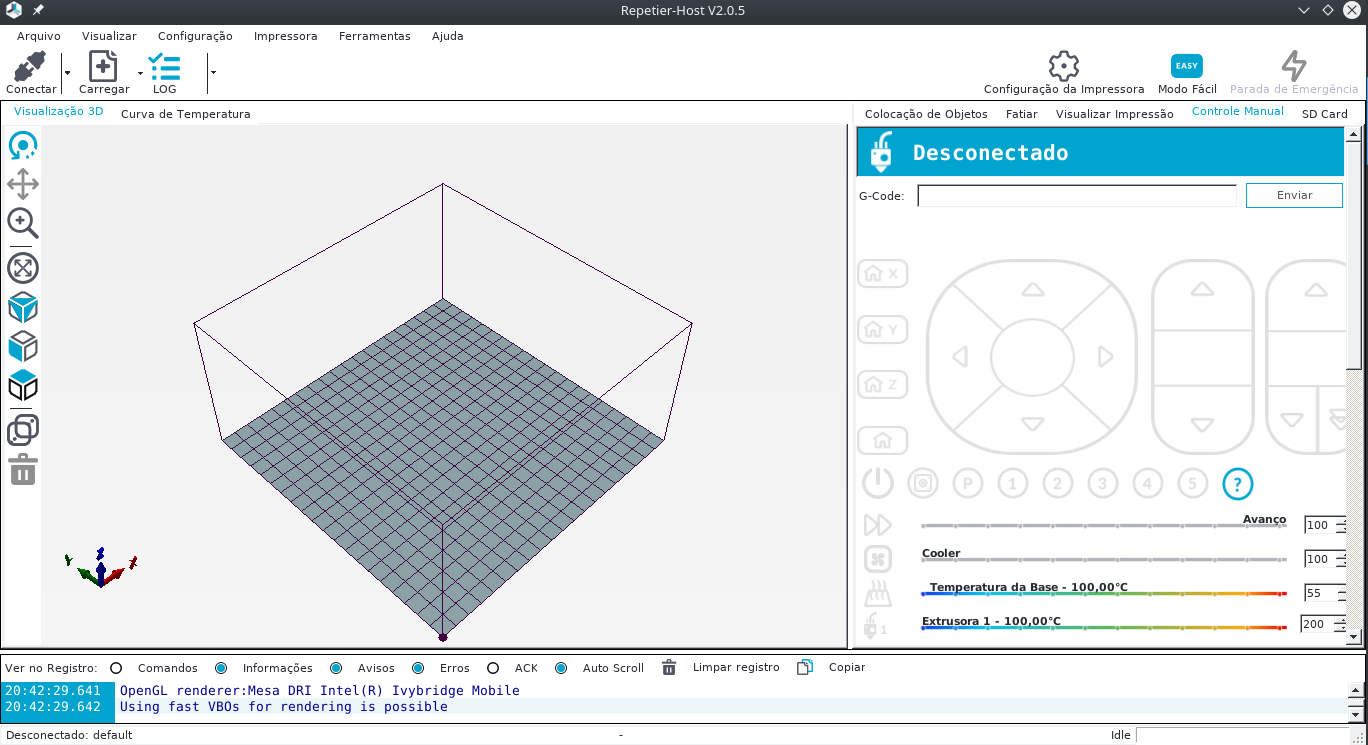
\includegraphics[width=\linewidth]{repetier}
\end{figure}

\subsubsection{OctoPrint}
O OctoPrint é um printer host criado para ser um host remoto, ou seja, ele possibilita
o gerenciamento remoto da Impressora 3D. Ele foi desenvolvido para ser um servidor remoto,
onde o usuário acessa um dispositivo com o OctoPrint instalado, normalmente um RaspberryPi,
e realiza o controle da impressora. Ao conectar a impressora 3D ao RaspberryPi ou
qualquer que seja o dispositivo que esteja servindo o OctoPrint, o usuário tem
acesso a ferramentas como o controle geral da impressora, monitoração de temperaturas,
ser informado através de 'Push Notifications' do status da impressora, além de possuir
 plugins que estendem suas funcionalidades. O OctoPrint possui seu código aberto
 sobre a licença AGPL, e foi criado pela desenvolvedora alemã Gina Häußge. A versão
 1.0.0 do OctoPrint foi lançada em 28 de Outubro de 2013 e nomento da escrita deste trabalho se encontra na versão 1.3.6.
Häußge escreveu o código do OctoPrint usando Python-Flask para a parte servidor, e HTML/JavaScript para o cliente.
\iffalse
Referências:
- Release: https://github.com/foosel/OctoPrint/releases
- Author: https://foosel.net/
- Licença: https://github.com/foosel/OctoPrint/blob/master/LICENSE
- Site: octoprint.org
- Features: https://octoprint.org/#full-remote-control-and-monitoring
https://octoprint.org/#compatible-and-extendable
\fi
\begin{figure}[H]
    \centering
    \caption[Octoprint]{Visão Geral do Octoprint}
    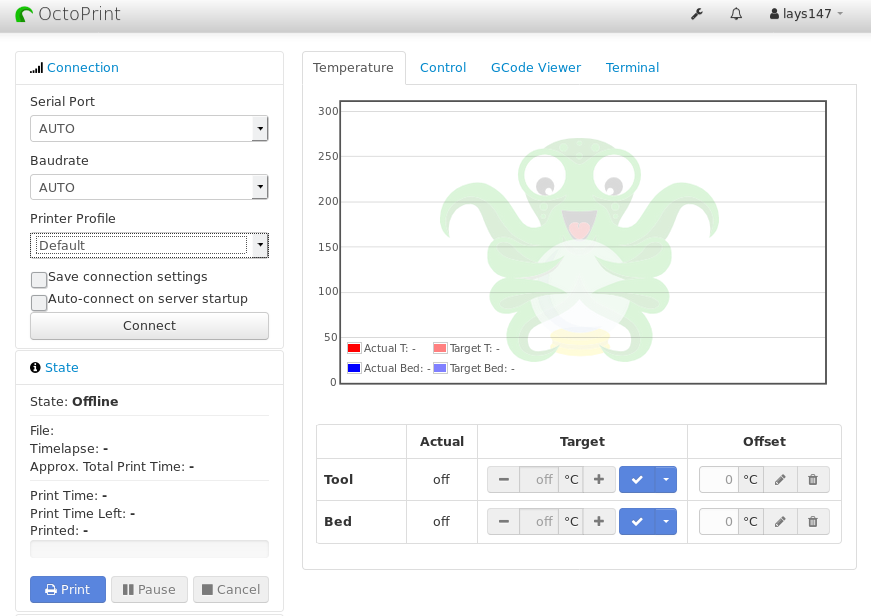
\includegraphics[width=\linewidth]{octoprint}
\end{figure}

\subsubsection{MatterControl}
O Matter Control é um printer host desenvolvido desde 2014 pela empresa MatterHackers sediada
na Califórnia, Estados Unidos. Em suas ferramentas se encontram a renderização do modelo em 3D,
gerenciamento geral da impressora e envios de SMS quando a impressão se conclui.
Possui seu código fonte aberto sobre a licença BSD 2-Clause e é 100\% escrito
com a linguagem de programação C\#. É uma aplicação multiplataforma, porém no ambiente
Linux é limitado as plataformas baseadas em distribuições Ubuntu ou Linux Mint, de acordo com os binários
disponibilizados em seu website. No momento da escrita deste trabalho, o Matter Control se encontra na versão 1.7.5.
\iffalse
Referências:
- Release: https://github.com/MatterHackers/MatterControl/tree/Releases
- Author: Matter Hackers
- Licença: https://github.com/MatterHackers/MatterControl/blob/master/LICENSE
- Site: https://www.matterhackers.com/mattercontrol
\fi

\begin{figure}[H]
    \centering
    \caption[Repetier Host]{Visão Geral do Matter Control}
    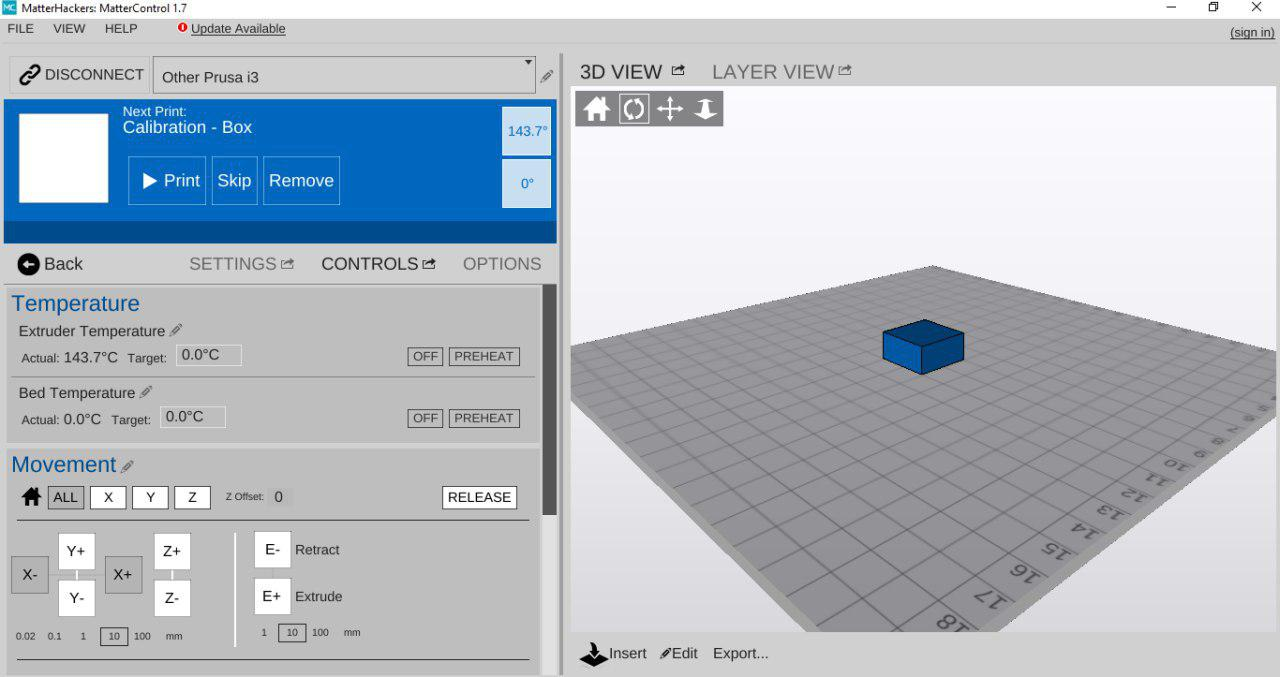
\includegraphics[width=\linewidth]{mattercontrol}
\end{figure}

\newpage
\section{Atelier}
\subsection{Motivação}
\subsection{Tecnologias Utilizadas}
\subsection{AtCore}
\subsection{Atelier}

\section{Análise Comparativa}
\subsection{Atelier x Repetier Host}
\subsubsection{Compatibilidade entre plataformas}
\subsubsection{Usabilidade}

\newpage
\section{Conclusão} 


\bibliography{bibliografia}

\end{document}
